\documentclass[11pt,a4paper]{article}
\usepackage[margin=0.80in]{geometry}
\usepackage{amsmath,amssymb,booktabs,multirow,graphicx,xcolor,siunitx,enumitem,hyperref,float,caption}
\hypersetup{colorlinks=true,linkcolor=black,citecolor=blue,urlcolor=blue}
\captionsetup{font=small}
\setlength{\parskip}{4pt}
\setlength{\parindent}{0pt}
\setlist{nosep}
\title{Controlled Small-Data Model Selection: A Reproducible Comparison of Classical Baselines, Grid Tuning, and Automated Search}
\author{Rachna Gupta\\ RSI2026510\\ AI Tools for Research --- Implementation Paper}
\date{17 November 2026}
\begin{document}
\maketitle
\begin{abstract}
A preceding literature review of expert-designed machine learning, conventional automated machine learning (AutoML), and language-model-driven agents identified validation instability, model-selection bias, and computing cost as major issues in small-data evaluation. We convert that broad review into a restricted, executable comparative study. Fixed logistic regression and random forest are compared with an inner-cross-validated radial-basis support vector machine (SVM) and Optuna-based random and tree-structured Parzen estimator (TPE) searches. All selected models share stratified inner validation folds, and the outer evaluation uses three stratified folds with two random seeds. Three genuinely tabular classification datasets constitute the primary analysis; a fourth image-derived feature-vector task is reported separately. Automated search is limited to 12 trials per fold and is not presented as a full AutoML package or an LLM agent. The recorded study contains 144 method evaluations and 17,964 held-out predictions; the audit program independently recomputes all performance metrics. Across the three primary tabular tasks, the highest observed mean balanced accuracy is 97.04\% obtained by Logistic regression, whereas the full four-task average is highest for TPE 12 at 96.95\%. These are descriptive findings, not claims of statistically significant or globally near-optimal performance. The study contributes a documented comparison protocol and an examination of search-budget and dataset-dependent behavior.
\end{abstract}
\textbf{Keywords:} small-data classification; automated hyperparameter search; nested cross-validation; SVM; Optuna; benchmarking; reproducibility.

\section{Introduction}
Selecting a machine-learning pipeline entails several decisions: how to preprocess features, which model family to use, which hyperparameters to search, which validation metric to optimize, and how to estimate performance on unseen data. These decisions can be especially consequential when training observations are scarce. An apparently advantageous setting can win a small validation comparison by chance, and repeated reuse of the same held-out sample can make reported performance overoptimistic. The distinction between model selection and unbiased evaluation is established in work on nested cross-validation \cite{varma2006}.

Our earlier review, \emph{Benchmarking AutoML and Agentic Pipelines Against Expert-Tuned Models on Small Datasets}, organized the literature into expert-designed pipelines, AutoML tools, LLM-guided agentic workflows, and specialized small-data models. That review proposed balancing predictive quality against stability, computational requirements, leakage control, and human effort. It did not implement or measure an experimental benchmark. The present implementation study takes one narrow part of that agenda and answers it with real measurements.

Standard automated machine-learning frameworks such as auto-sklearn and FLAML seek good configurations while reducing user intervention \cite{feurer2015,wang2021}. The AMLB project illustrates the need for common evaluation conditions and multiple reporting dimensions \cite{gijsbers2024}. A full comparison across expert researchers, established AutoML packages, and autonomous LLM agents would require carefully controlled human time, model-access conditions, external retrieval, extensive computational resources and multiple agent reruns. None of these is silently assumed here. Instead, we evaluate a small, inspectable model-selection component using Optuna, a published optimization library \cite{akiba2019}, against fixed and grid-tuned machine-learning controls.

\textbf{Study question.} Given the same outer test folds and inner cross-validation folds, does a 12-trial automated search provide useful predictive gains relative to a carefully specified tuned SVM and to random search, and how do results change with task characteristics and search budget? Our goal is a reproducible course-scale experiment, not a declaration that any search algorithm is best across all data regimes.

\section{Literature-to-Experiment Bridge}
\subsection{Sources and rationale}
The existing review highlighted that AutoML tools are not interchangeable. Their search spaces, computational budgets, and defaults differ, so simply naming an AutoML tool does not determine its evaluation protocol. The published AMLB benchmark supports standardizing data access and failure reporting \cite{gijsbers2024}; the nested-CV literature supports separation of selection and assessment \cite{varma2006}. The Optuna framework supplies random and model-based samplers suitable for a controlled optimizer comparison \cite{akiba2019}. These original publications support the experimental design, but do not demonstrate that the precise comparison here is novel or that our measured differences will generalize.

Our earlier review also discussed TabPFN, an in-context tabular classification model \cite{hollmann2023}, and AutoML-Agent, an LLM-based automated workflow \cite{trirat2025}. They are relevant comparators for a future, broader benchmark, but are \emph{not} executed in the current study. This is an explicitly narrowed comparative pathway, consistent with the assignment's allowance for controlled comparisons and informative negative results.

\subsection{Questions and intended measurements}
\begin{description}
\item[RQ1 --- Generalization:] How do fixed logistic regression, fixed random forest, grid-tuned SVM, random search and TPE search compare on held-out balanced accuracy and macro-F1?
\item[RQ2 --- Optimizer control:] Under the same 12-trial candidate budget and search space, does the TPE-based selection achieve different held-out behavior from uniform random sampling?
\item[RQ3 --- Budget sensitivity:] What happens when the TPE study continues from its first four startup trials to 12 total trials?
\item[RQ4 --- Operational cost:] What additional observed fit/search time is associated with the candidate-search methods? Does the ranking vary across datasets?
\end{description}
All primary metrics, fold construction, and candidate configurations were fixed in the source implementation; reported scores are obtained from test folds that are not used for parameter selection.

\section{Experimental Design and Implementation}
\subsection{Data and task profile}
We use datasets distributed with scikit-learn \cite{pedregosa2011}; their source objects are loaded programmatically, rather than manually copied into the manuscript. The three primary tabular tasks are Breast Cancer Wisconsin (Diagnostic), Wine, and Iris. We additionally study a stratified 600-observation subset of handwritten Digits, retaining its 64 flattened image-pixel features. Digits is an \emph{auxiliary feature-vector classification task}, not an ordinary tabular dataset; therefore results averaged over all four tasks are not interpreted as a tabular-only benchmark.

\begin{table}[H]
\centering\caption{Datasets recorded by the implemented loader. All training folds contain no more than 1,000 observations.}
\small
\begin{tabular}{lrrrl}\toprule
Task & Total rows & Features & Classes & Study role\\\midrule
Breast Cancer & 569 & 30 & 2 & Primary tabular\\
Wine & 178 & 13 & 3 & Primary tabular\\
Iris & 150 & 4 & 3 & Primary tabular\\
Digits600 & 600 & 64 & 10 & Supplementary image vectors\\\bottomrule
\end{tabular}
\end{table}

For Digits600, the subset is selected by a single stratified sampling operation using seed 42 \emph{before} outer CV. For every task, the original rows and target labels are otherwise unchanged. The selected sample sizes are a practical demonstration of the review's operational small-data regime, not a universally accepted threshold. No patient, group or temporal metadata are assumed; task-specific grouped validation is outside the current scope.

\subsection{Outer and inner evaluation folds}
For each task we repeat stratified three-fold cross-validation with random seeds 42 and 123. Denote the $j$-th outer training and test sets by $D_{\mathrm{train}}^{(j)}$ and $D_{\mathrm{test}}^{(j)}$. The full hyperparameter selection process is restricted to the outer training subset:
\begin{equation}
\hat\lambda^{(j)}=\underset{\lambda\in\Lambda}{\arg\max}\;\frac{1}{3}\sum_{k=1}^{3}
\mathrm{BAcc}\bigl(f_{\lambda}^{(j,k)},D_{\mathrm{val}}^{(j,k)}\bigr),
\end{equation}
where the inner training and validation splits derive solely from $D_{\mathrm{train}}^{(j)}$. The selected method is refitted on all outer training rows and produces one prediction for each sample in $D_{\mathrm{test}}^{(j)}$. For each dataset and seed, every sample belongs to exactly one test fold; folds overlap in training data, so their results are \emph{not statistically independent experimental replications}.

The same prespecified inner fold indices are provided to GridSearchCV, Optuna random search, and Optuna TPE search. Standardization is inside the scikit-learn estimator pipeline, so the mean and scale of any held-out test sample cannot influence training or tuning. This prevents a common preprocessing leakage error.

\subsection{Model configurations and candidate budgets}
The baseline set contains (i) logistic regression with StandardScaler and $C=1$, (ii) a random forest with 150 trees, default leaf size, and fixed seed, and (iii) an RBF SVM with StandardScaler. The SVM is selected using $C\in\{0.1,1,10,100\}$ and $\gamma\in\{\mathrm{scale},0.01,0.1\}$, giving 12 grid candidates evaluated through common three-fold inner CV. These choices constitute a \emph{protocol-defined tuned baseline}; they are not evidence of time spent by a human subject or of globally optimized SVM hyperparameters.

For automated selection, Optuna samples either an RBF SVM or a random forest. SVM uses $C\in[10^{-2},10^{3}]$ on a logarithmic scale and $\gamma\in\{\mathrm{scale},10^{-4},10^{-3},10^{-2},10^{-1},1\}$. Forest candidates use 60 or 100 trees, max depth from \{unbounded, 5, 10\}, and minimum leaf size from \{1,2\}. The search space is deliberately modest and fully recorded in the source. It does not include feature-engineering agents, XGBoost or all candidate families used by established AutoML suites.

Two Optuna samplers search the \emph{same space} for 12 completed trials: RandomSampler and TPESampler. For TPE, the first four trials are explicitly random startup trials. The retained four-trial result (TPE4) is the best configuration at that point; TPE12 is the best configuration after all 12 trials. Thus TPE4 is a \emph{search-budget prefix}, not evidence of TPE's model-based selection. The 12-trial samplers are comparable in number of attempted configurations, but not necessarily in wall-clock time because candidate models differ.

\subsection{Metrics and data provenance}
Let $K$ be the number of target classes and $TP_c,FN_c$ the true positives and false negatives for class $c$. The primary metric is balanced accuracy:
\begin{equation}
\mathrm{BAcc}=\frac{1}{K}\sum_{c=1}^{K}\frac{TP_c}{TP_c+FN_c}.
\end{equation}
Macro-F1 and ordinary accuracy are recorded as secondary measures; measured elapsed search/refit time is recorded with a monotonic wall clock. Timing includes only fitting for fixed baselines, but includes the full inner parameter search plus the final refit for tuned methods. These totals describe practical workflow cost rather than compute-equalized training effort.

The benchmark writes each test prediction with dataset, seed, fold, method, original row index, true label and predicted label. It also saves trial-level inner scores and suggested configurations, fold-level scores, library versions and a console log. A separate verification program recomputes metrics from the raw prediction CSV, rejects duplicate test rows, verifies shared fold membership, checks complete test coverage per seed and method, and counts trial records. These are checks of the implementation artifacts, not an independent scientific replication.

\section{Measured Results}
\subsection{Primary tabular-only comparison}
Table~\ref{tab:tabular} summarizes the three genuine tabular tasks only. The entries are macro-averages of fold-level balanced accuracy, not pooled confusion-matrix accuracy; because all tasks use the same six held-out fold evaluations, each task receives equal weight in the descriptive aggregate.

\begin{table}[H]
\centering\caption{Primary tabular-only descriptive results over three datasets and six held-out folds per task. Standard deviation pools correlated repeated folds and is not a confidence interval.}
\label{tab:tabular}
\small\begin{tabular}{lrrrr}\toprule
Method & Bal. acc. & SD & Macro-F1 & Time (s)\\\midrule
Logistic regression & 97.04\% & 2.75\% & 97.08\% & 0.003 \\
Random forest & 96.26\% & 2.61\% & 96.27\% & 0.139 \\
Tuned SVM & 96.45\% & 2.28\% & 96.50\% & 0.109 \\
Random 12 & 96.37\% & 2.37\% & 96.49\% & 1.289 \\
TPE prefix 4 & 96.37\% & 1.90\% & 96.35\% & 0.653 \\
TPE 12 & 96.99\% & 1.81\% & 97.00\% & 1.289 \\
\bottomrule\end{tabular}
\end{table}

Across the three tabular tasks, the fixed logistic-regression baseline attains 97.04\% mean balanced accuracy, with TPE12 close at 96.99\% and grid-tuned SVM at 96.45\%. The difference between the two highest tabular-only means is only 0.05 percentage points. The result should not be interpreted as a proof that any procedure is universally preferable: the specific data conditions and tuning scope determine the ordering.

\subsection{Per-task outcomes}
Table~\ref{tab:perdataset} reports the observed mean balanced accuracy for each method and task. We report the supplementary Digits task alongside, while keeping its role explicit.

\begin{table}[H]
\centering\caption{Mean held-out balanced accuracy (percent) by method and task, with two seeds and three folds per seed.}
\label{tab:perdataset}
\scriptsize\setlength{\tabcolsep}{3pt}
\begin{tabular}{lrrrrrr}\toprule
Task & Logistic & RF & Tuned SVM & Rand12 & TPE4 & TPE12\\\midrule
Breast Cancer & 97.14 & 95.21 & 96.78 & 96.24 & 96.34 & 97.09\\
Wine & 98.61 & 98.55 & 97.52 & 97.17 & 97.05 & 97.52\\
Iris & 95.36 & 95.02 & 95.04 & 95.71 & 95.71 & 96.36\\
Digits600 (aux.) & 94.52 & 95.83 & 96.34 & 96.43 & 95.67 & 96.84\\
\bottomrule\end{tabular}
\end{table}

Figure~\ref{fig:perdataset} shows both means and descriptive between-fold standard deviations. The variability comes from six test-fold evaluations per task (three folds for two resampling seeds), not from independent datasets or repeated laboratory participants.

\begin{figure}[H]
\centering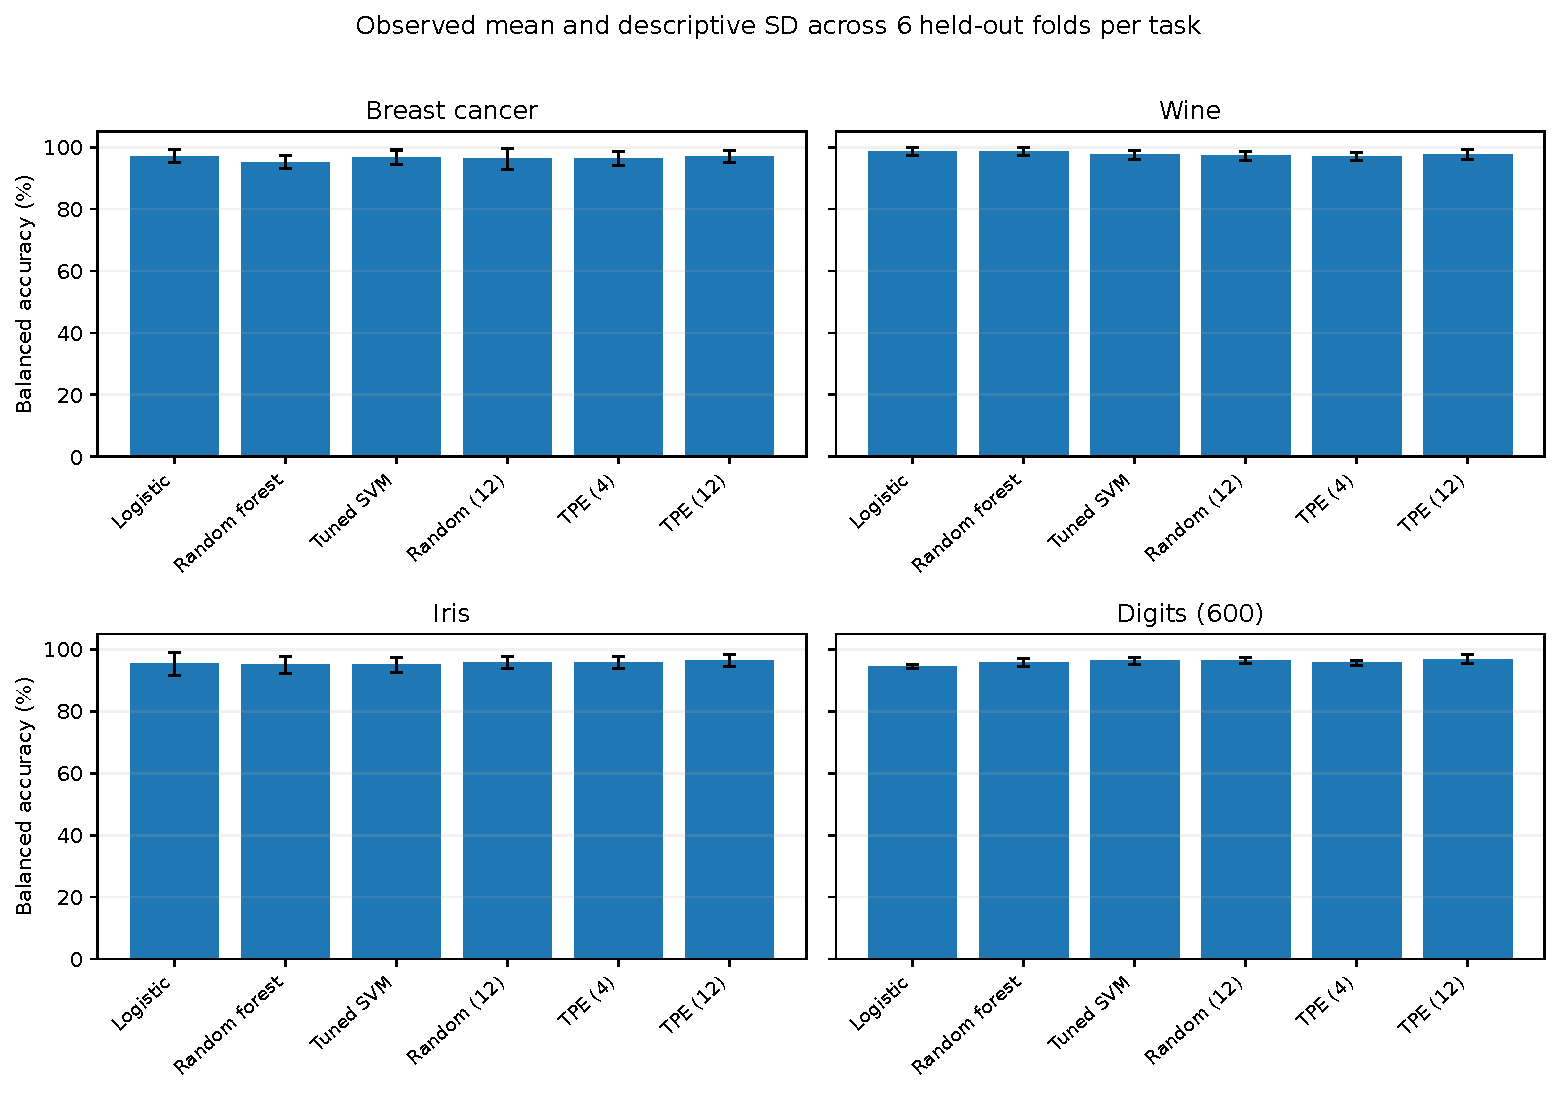
\includegraphics[width=\linewidth]{../results/figures/per_dataset_accuracy.pdf}
\caption{Observed balanced accuracy and descriptive standard deviation on four classification tasks. The Digits task is supplementary because its features originate from images.}
\label{fig:perdataset}
\end{figure}

\subsection{Overall four-task comparison and runtime}
Table~\ref{tab:overall} gives the complete four-task descriptive summary, including the supplementary feature-vector task. Its ranking must not be substituted for the tabular-only ranking.

\begin{table}[H]
\centering\caption{Four-task descriptive summary including the supplementary Digits600 feature-vector task (24 test folds per method).}
\label{tab:overall}
\small\begin{tabular}{lrrrr}\toprule
Method & Bal. acc. & SD & Macro-F1 & Time (s)\\\midrule
Logistic regression & 96.41\% & 2.63\% & 96.44\% & 0.004 \\
Random forest & 96.15\% & 2.34\% & 96.16\% & 0.151 \\
Tuned SVM & 96.42\% & 2.03\% & 96.46\% & 0.159 \\
Random 12 & 96.39\% & 2.09\% & 96.47\% & 1.389 \\
TPE prefix 4 & 96.19\% & 1.72\% & 96.18\% & 0.701 \\
TPE 12 & 96.95\% & 1.70\% & 96.96\% & 1.351 \\
\bottomrule\end{tabular}
\end{table}

The reported runtimes depend on the local CPU environment and on the number and type of model fits. SVM grid tuning evaluates 12 candidates, and each automated 12-trial study evaluates 12 configurations; however, candidate evaluations have unequal computational cost. Fixed logistic regression and fixed random forest are necessarily much cheaper because they perform no inner selection. Figure~\ref{fig:tradeoff} displays the observed tradeoff without claiming that all methods received a matched wall-clock budget.

\begin{figure}[H]
\centering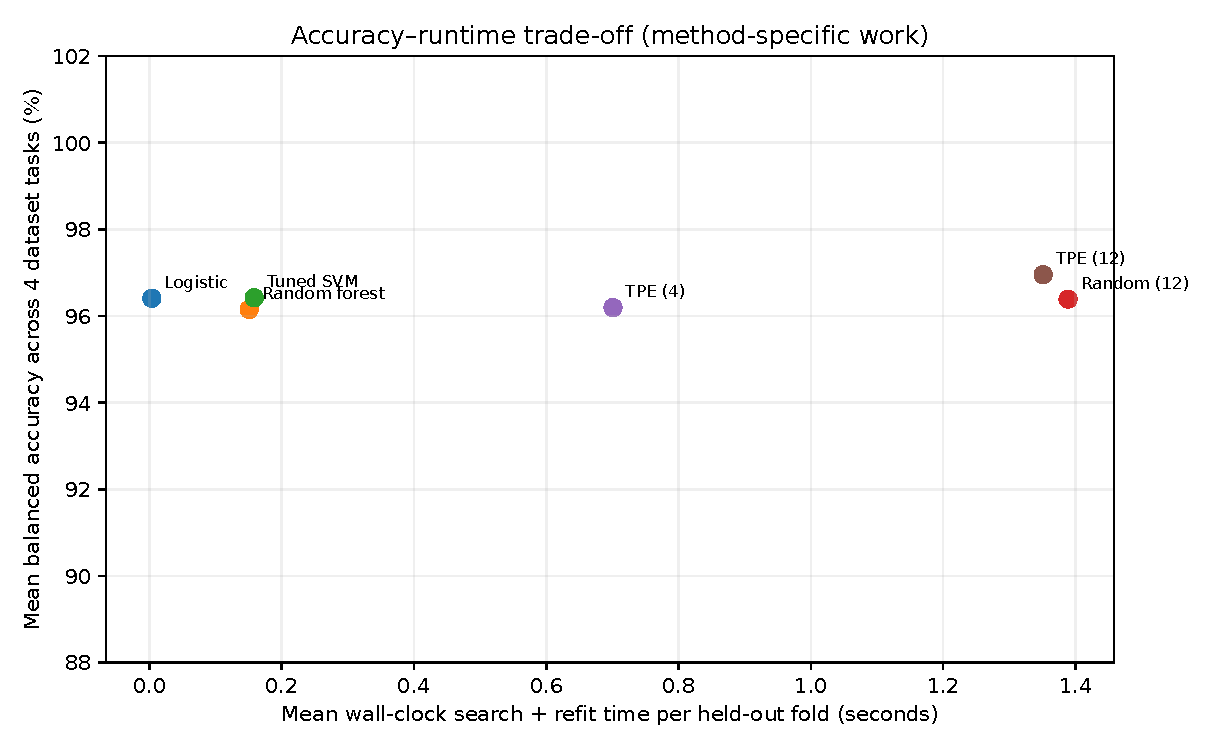
\includegraphics[width=.82\linewidth]{../results/figures/runtime_tradeoff.pdf}
\caption{Observed four-task balanced accuracy against per-fold measured search-and-refit time. Times are machine-dependent and baseline methods perform unequal amounts of selection work.}
\label{fig:tradeoff}
\end{figure}

\section{Deeper Analysis: Search Budget and Optimizer Choice}
\subsection{Equal-trial random versus TPE sampling}
Random12 and TPE12 use identical candidate families, parameter bounds, seed-dependent inner folds and a budget of 12 trials. Their differences arise from the sampler strategy and the particular configurations drawn. TPE12 attains 96.95\% on the full four-task summary versus 96.39\% for Random12, a descriptive difference of 0.56 percentage points. The difference relative to grid-tuned SVM is 0.53 percentage points. Both search procedures have 12 trials, but their candidate configurations and runtime realizations differ. Even an observed positive advantage on one dataset would not show that TPE is asymptotically superior or near-optimal under all settings: 12 trials is a limited local search.

\subsection{Within-study budget extension}
To separate an early random-initialization phase from later model-based suggestions, we retain the best configuration after four TPE-study trials and again after 12. A higher best \emph{inner} score at trial 12 is guaranteed by how best-so-far selection works, but a higher held-out \emph{outer} score is not guaranteed. Figure~\ref{fig:budget} presents the actual held-out changes, including zero and negative outcomes when present.

\begin{figure}[H]
\centering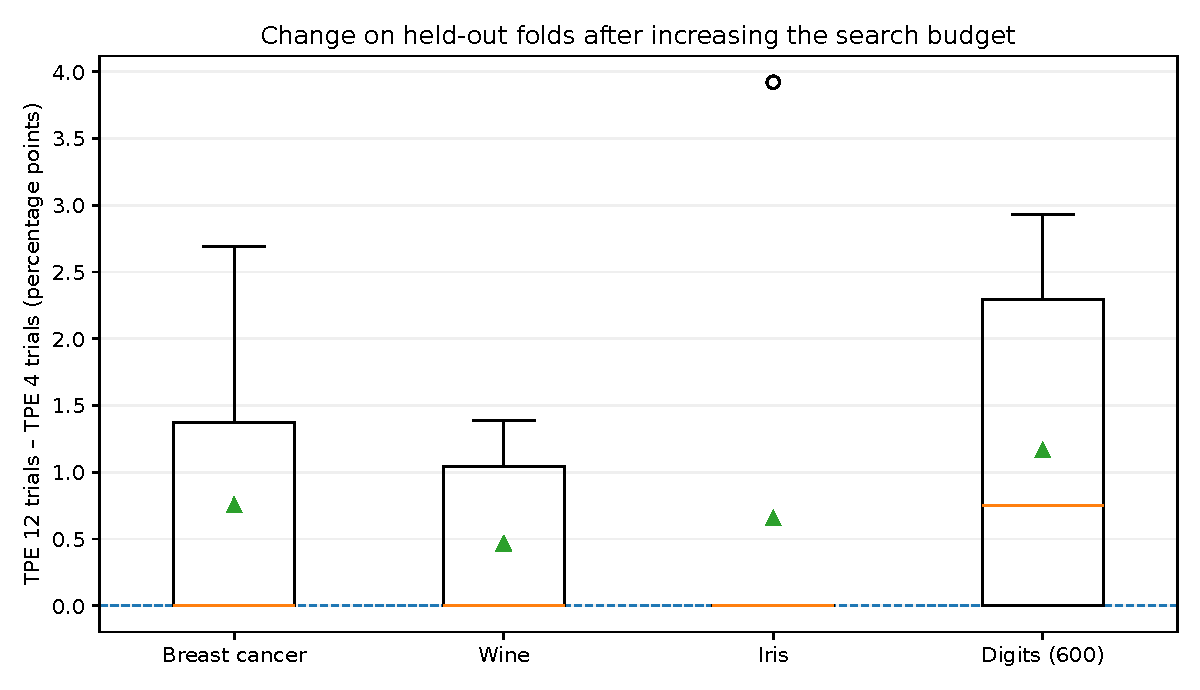
\includegraphics[width=.82\linewidth]{../results/figures/budget_effect.pdf}
\caption{Within-study change in held-out balanced accuracy from the four-trial startup prefix to the complete 12-trial TPE study. A zero change can mean the previously selected configuration remained optimal on inner CV.}
\label{fig:budget}
\end{figure}

The twelve-trial TPE search improves over its four-trial prefix in 8 of the 24 matched test-fold comparisons, ties in 16, and is lower in 0; the aggregate difference is 0.76 percentage points. This is a within-study observational budget comparison, not a formal proof that more trials always improve generalization. This comparison is informative precisely because more optimization opportunities do not mechanically imply a better independent-test result.

\subsection{Dataset dependence and failure modes}
The primary tabular tasks are not won by the same method on every dataset: mean balanced accuracy is highest for logistic regression on Breast Cancer (97.14\%) and Wine (98.61\%), while TPE12 is highest for Iris (96.36\%). On the supplementary Digits task TPE12 also leads (96.84\%). These descriptive differences show why tabular-only and auxiliary summaries should be reported separately. Errors can arise from limited validation observations, search-space imbalance, constrained trial budgets, or learner--task mismatch. The current data do not isolate those mechanisms causally. No unmeasured feature-importance explanation, significance claim or test-set-driven tuning decision is introduced to rationalize an unfavorable result.

\section{Threats to Validity}
\textbf{Small benchmark collection.} Only three genuine tabular datasets are used as the primary set, plus one image-derived feature-vector task. All are relatively clean, numerical, and distributed with a mainstream library. They do not capture sparse categorical inputs, severe missingness, major distribution shift, or data with group-wise dependence.\par
\textbf{Dependence among resamples.} Two outer seeds and three folds per seed make six test estimates per task but not six statistically independent samples. We therefore report descriptive standard deviations and avoid inferential $p$-values or overstated confidence intervals. A stronger study would use many more independent datasets.\par
\textbf{Search and tuning budgets.} Optuna has only 12 trials per outer fold, with two model families. The SVM grid and sampler strategies do not have equal CPU budgets despite similar candidate counts. Scores cannot establish global optimum configurations or a reliable superiority ordering among professional AutoML packages.\par
\textbf{Methodological scope.} The study neither implements nor evaluates an LLM agent, auto-sklearn, FLAML, TabPFN or an externally evaluated human expert. A tuned RBF-SVM does not operationalize professional expertise by itself. Therefore the paper answers a scoped subset of the original review's questions and must not be titled as an empirical expert--AutoML--agent study.\par
\textbf{Runtime measurement.} Wall-clock measurements were collected on a single Linux CPU environment and may be sensitive to background processes and software versions. No energy, monetary API, or human participant time was measured.\par
\textbf{Possible prior data exposure.} Standard library benchmark datasets are widely used and model development on them is not a blind competition; our protocol freezes outer test subsets for this run, but it cannot erase prior knowledge of their general properties.\par

\section{Reproducibility and Human--AI Accountability}
The package provides the exact executable source, retained run log from the completed benchmark, an environment manifest, JSON settings, three levels of CSV outputs, and both vector and raster figures. To regenerate the recorded outputs, install the dependency requirements, limit BLAS threads for closer timing comparability if desired, execute \texttt{python src/benchmark.py --seeds 42 123 --trials 12}, and run \texttt{python src/verify\_outputs.py} followed by \texttt{python src/plots.py}. The validation program returned \texttt{PASS} for 144 method evaluations and 17,964 test predictions. Timing and possibly marginal scores may vary when dependencies or hardware change.

AI-assisted code generation, file inspection, result verification, figure creation and manuscript drafting were performed in this research-workflow interaction. The authorship/provenance log distinguishes what was executed here from tasks the student must personally repeat or defend. The instructor-requested similarity/plagiarism and AI-writing detection reports for the review and implementation paper are distinct external documents that must be obtained from an accepted service; no such scores are inferred or fabricated by the benchmark.

\section{Conclusion}
We transformed a broad small-data AutoML and agentic-learning review into a narrowly defined executable model-selection comparison. A shared nested-validation design, two seeds, matched-fold 12-trial samplers, prediction-level audit trail and recorded runtimes permit a more reliable descriptive comparison than a single attractive accuracy figure. Among the three primary tabular tasks, simple fixed logistic regression is the highest-scoring method on the macro-averaged balanced-accuracy metric (97.04\%), narrowly above TPE12 (96.99\%). Over all four tasks, TPE12 attains the largest mean (96.95\%), but at higher observed fit/search time than tuned SVM and far higher time than the fixed logistic baseline. These rankings depend on the inclusion of the supplementary image-derived dataset and must not be presented as universal performance superiority. The findings are conditioned on the available datasets and budgets. A useful next study would examine more OpenML tabular tasks, additional random seeds, a properly implemented full AutoML tool, and an actual agentic workflow with documented model access and intervention costs. Such extensions are not claimed as completed here.

\clearpage
\begin{thebibliography}{9}
\bibitem{varma2006} S. Varma and R. Simon, ``Bias in error estimation when using cross-validation for model selection,'' \emph{BMC Bioinformatics}, vol. 7, art. 91, 2006. doi:10.1186/1471-2105-7-91.
\bibitem{akiba2019} T. Akiba, S. Sano, T. Yanase, T. Ohta and M. Koyama, ``Optuna: A Next-generation Hyperparameter Optimization Framework,'' in \emph{Proc. ACM SIGKDD}, 2019. doi:10.1145/3292500.3330701.
\bibitem{gijsbers2024} P. Gijsbers \emph{et al.}, ``AMLB: an AutoML Benchmark,'' \emph{J. Machine Learning Research}, vol. 25, no. 101, pp. 1--65, 2024.
\bibitem{feurer2015} M. Feurer \emph{et al.}, ``Efficient and Robust Automated Machine Learning,'' in \emph{Advances in Neural Information Processing Systems}, vol. 28, 2015.
\bibitem{wang2021} C. Wang, Q. Wu, M. Weimer, and E. Zhu, ``FLAML: A Fast and Lightweight AutoML Library,'' in \emph{Proc. Machine Learning and Systems}, vol. 3, pp. 434--447, 2021.
\bibitem{hollmann2023} N. Hollmann, S. Muller, K. Eggensperger, and F. Hutter, ``TabPFN: A Transformer That Solves Small Tabular Classification Problems in a Second,'' in \emph{ICLR}, 2023.
\bibitem{trirat2025} P. Trirat, W. Jeong, and S. J. Hwang, ``AutoML-Agent: A Multi-Agent LLM Framework for Full-Pipeline AutoML,'' in \emph{Proc. ICML}, vol. 267, pp. 60099--60146, 2025.
\bibitem{pedregosa2011} F. Pedregosa \emph{et al.}, ``Scikit-learn: Machine Learning in Python,'' \emph{J. Machine Learning Research}, vol. 12, pp. 2825--2830, 2011.
\end{thebibliography}
\end{document}
